% This is samplepaper.tex, a sample chapter demonstrating the
% LLNCS macro package for Springer Computer Science proceedings;
% Version 2.20 of 2017/10/04
%
\newcommand{\antonio}[1]{\textcolor{red}{#1}}
%
\documentclass[runningheads]{llncs}
%
\usepackage{graphicx}
\usepackage{multirow}
\usepackage{amsfonts}
\usepackage[table,xcdraw]{xcolor}
\usepackage{subfigure}

% Used for displaying a sample figure. If possible, figure files should
% be included in EPS format.
%
% If you use the hyperref package, please uncomment the following line
% to display URLs in blue roman font according to Springer's eBook style:
% \renewcommand\UrlFont{\color{blue}\rmfamily}
%
\begin{document}
%
\title{Geographic Context-Based Stacking Learning for Election Prediction from Socio-Economic Data\thanks{This study was financed in part by the Coordena{\c{c}}\~{a}o de Aperfei{\c{c}}oamento de Pessoal de N\'{i}vel Superior -- Brasil (CAPES) -- Finance Code 001.}}
%
\titlerunning{Stacking Learning for Election Prediction from Socio-Economic Data}
% If the paper title is too long for the running head, you can set
% an abbreviated paper title here
%
\author{Tiago Pinho da Silva\inst{1}\orcidID{0000-0001-9381-0982} \and
Antonio R. S. Parmezan\inst{1}\orcidID{0000-0002-1725-132X} \and
Gustavo E. A. P. A. Batista\inst{2}\orcidID{0000-0002-3482-8442}}
%
\authorrunning{da Silva et al.}
% First names are abbreviated in the running head.
% If there are more than two authors, 'et al.' is used.
%
\institute{University of S\~{a}o Paulo, S\~{a}o Carlos, Brazil
%\email{\{tpinho,parmezan\}@usp.br}
\and
University of New South Wales, Sydney, Australia}
%\email{g.batista@unsw.edu.au}}
%
\maketitle % typeset the header of the contribution
%
\begin{abstract}
Voting behavior analysis involves understanding factors influencing an election to identify possible trends, new features, and extrapolations. A growing body of research has joined efforts to automate this process from high-dimensional spatial data. Although some studies have investigated machine learning methods, the capability of this artificial intelligence subarea has not been fully explored due to the challenges posed by the spatial autocorrelation structure prevalent in the data. This paper advances the current literature by proposing a geographic context-based stacking learning approach for predicting election outcomes from census data. Our proposal models data in spatial contexts of different dimensions and operates on them at two levels. First, it captures local patterns extracted from spatial contexts. Then, at the meta-level, it globally captures information from the $K$ contexts nearest to a region we want to predict. We introduce a spatial cross-validation-driven experimental setup to assess and compare the stacking approach with state-of-the-art methods fairly. This validation mechanism aims to diminish spatial dependence's influence and avoid overoptimistic results. We estimated a considerable multi-criteria performance of our proposal concerning baseline and reference models taking data from the second round of the 2018 Brazilian presidential elections into account. The stacking approach presented the best overall performance, being able to generalize better than the compared ones. It also provided intelligible and coherent predictions in challenging regions, emphasizing its interpretability. These results evidence the potential use of our proposal to support social research.

\keywords{Ensemble Learning, Metalearning, Preferential Voting, Spatial Dependence, Voting Behavior.}
\end{abstract}


%%

\section{Introduction}

Elections are non-trivial processes essential to any representative democracy, which can provide the best expression of public opinion and party involvement. A post-election data analysis allows us to describe voting behavior and the aspects that guide it \cite{lucas2020}. Understanding voting behavior is vital to identifying trends and factors influencing election results \cite{layton2021demographic,pinheiro2020hope}.

Researchers consider that the electoral processes are associated with the population characteristics regarding the locations where they occur. Thus, an electoral process comprises aspects that indicate local patterns related to spatial autocorrelation and local relationships across space \cite{stewart2021scale}. In this perspective, people from the same region tend to present similar voting behavior, while those from distinct areas may have different vote distributions.

Considering how people are geographically contextualized and the data's spatial characteristics can enrich our understanding of electoral processes. We have witnessed an increasing number of interdisciplinary studies aimed at predictive modeling election features from thousands of explanatory spatial features \cite{tiago2021graph,li2019deep}. However, the high dimensionality and spatial autocorrelation structure inherent in such data limit the ability of conventional learning models to capture the relationships between spatial features completely.

Many econometric and machine learning methods, which can deal with the curse of dimensionality, totally ignore the geography present in electoral data, such as spatial boundaries, clustering effects, and distance measures \cite{graefe2019accuracy,chauhan2021emergence}. Consequently, they treat data separated into regions as independent and identically distributed. In the opposite direction, recent studies have suggested using spectral and spatial filtering Graph Convolutional Neural Network (GCNN) methodologies to enrich election data modeling \cite{li2019deep}. Such methods seem to adequately fit the problem at hand, given the intrinsic graph structure of electoral data.
% Although these models can lead to accurate results within a reasonable number of iterations, as verified in \cite{li2019deep} with the Hierarchical GCNN, they are complex and expensive.

This work advances the literature on voting behavior analysis by proposing a geographic context-based stacking learning approach to describe election outcomes from thousands of census features. Our proposal models data in spatial contexts of different dimensions and operates on them at two levels: (i)~at the base level, it captures local patterns extracted from spatial contexts; (ii)~at the meta-level, it globally captures information from the $K$ contexts nearest to a region we want to predict. %Although we build a predicting model, we are strictly interested in the patterns learned by the model to provide insights towards election outcomes. 
Furthermore, we introduce a spatial cross-validation-driven experimental setup to assess and compare the stacking approach with state-of-the-art methods fairly. This validation mechanism can generate robust assessments by diminishing the spatial dependence's influence and consequently avoiding overoptimistic results \cite{tiago2021graph,ploton2020}.

We estimated a considerable multi-criteria performance of our proposal concerning two baselines and the state-of-the-art Hierarchical GCNN method taking data from the second round of the 2018 Brazilian presidential elections into account. The stacking approach exhibited the best overall performance, being able to generalize better than the compared ones. It also led to intelligible and coherent predictions in challenging regions, highlighting its interpretability. These results demonstrate the potential use of our proposal to support social research.

The rest of this paper is organized as follows: Section~\ref{sec:relatedwork} introduces the background and related work. Section~\ref{sec:proposed_approach} describes our geographic context-based stacking learning approach. Section~\ref{sec:case_study} reports the case study involving data from the second round of the 2018 Brazilian presidential election. Finally, Section~\ref{sec:conclusion} concludes the study and highlights future work.


%%

\section{Background and Current Trends}
\label{sec:relatedwork}

This section defines the mathematical notation that models election voting behavior considering the spatial characteristics of the data. It also discusses related work covering the most recent advances in the literature.

%%

\subsection{Problem Definition and Research Challenges}
\label{subsec:problem_definition}

We can formulate the problem in question as follows. First, let us specify a set of lattice-type spatial objects $O$, where each object $o_i$ is a polygon that delimits a region in the spatial domain (\textit{e.g.}, neighborhoods, districts and cities). Note that the spatial intersection between any distinct objects $o_i$ and $o_j \in O$ is the empty set ($\emptyset$). Now, let us assume a spatial dataset $D = \{X,Y\}$ that characterizes each of the $n$ objects in $O$. The target feature, $Y \in \mathbb{R}$, reflects the vote shares (vote percentage) for each spatial object in $O$ from a given candidate or party. The explanatory features, $X \in \mathbb{R}^m$, where $m > 0$ is the number of characteristics, describes the spatial objects from $O$ in another election-related domain. Let us also consider a set of spatial contexts $C$ with boundaries that segment $D$ in the geographic space, where $C$ can be defined based on preexisting boundaries (\textit{e.g.}, states and macro-regions). The objective is to generate a model $F(D,C)$ that learns local relationship patterns from the spatial contexts present in $D$. %Illustratively, $O$ can be the set of cities ($o_i$), such that  $Y \in \mathbb{R}$ is the outcome space containing vote shares distribution for a given candidate, and $X \in \mathbb{R}$ is the explanatory feature space presenting demographic information for the cities. Moreover, the spatial contexts $C$ can be defined as the states. It is noteworthy that the spatial contexts can be defined by any group of geographic boundaries with overlapping or not.

Modeling local relationships between explanatory features and the target feature (vote shares) is not a trivial task. These relationships may vary across spatial contexts, meaning that a relevant characteristic that can describe the vote shares from one context may not be useful to another \cite{stewart2021scale}. Furthermore, in a conventional machine learning approach, local relationships are disregarded in favor of those that describe the vote shares globally \cite{tiago2021graph,stewart2021scale}. % In other words, the conventional approach preferred features that can explain most of the data. Thus, not using features that are good for describing a small part of the data since they are not useful for the remaining data.

Another challenge in modeling voting behavior relates to using Spatial Cross-Validation~(SCV) as a sampling technique. While it is the most suitable procedure for assessing machine learning models built from spatial data, it generates unseen correlated distributions in the test set. This scenario happens because spatial boundaries determine the folds, and a removing buffer region is defined as a strategy to diminish the spatial dependence between the test and training sets \cite{tiago2021graph,ploton2020}. Consequently, the test set distribution is not observed in the training set, and there are only correlated distributions.

%Therefore, modeling electoral voting behavior using machine learning methods is not a trivial task. In Section~\ref{sec:proposed_approach}, we discuss how to cope with such challenges.

Studies on applying machine learning methods for analyzing voting behavior are maturing through scientific debate. Section~\ref{subsec:related_work} briefly summarizes some related work in this field, emphasizing the challenges they brought.

%In this work, we define unseen correlated distributions as those that do not appear in the training set but present a certain level of correlation with the training set such that the model can still provide good predictions. An example in our applications happens when we try to predict the vote shares from the Northeast region. We do not observe the distribution of votes and explanatory features from the Northeast in the remaining regions. They are, in a particular manner, exclusive from this region. However, we still have correlated distributions, especially in the North, to predict the vote shares from the Northeast.

%%

\subsection{Related Work}
\label{subsec:related_work}

The vast literature on voting behavior varies from standard econometric techniques \cite{graefe2019accuracy} to regression analysis \cite{stewart2021scale} and machine learning models \cite{chauhan2021emergence,li2019deep}. Econometrics and regression analysis studies usually focus on national-level estimators using surveys and economic features to understand election results. Although these methods are well established \cite{graefe2019accuracy}, applying them to thousands of features in several locations is challenging. Conversely, machine learning models can deal with the curse of dimensionality more naturally. However, most works employs social media data and sentiment analysis to understand voting behavior. Their results are commonly explored on a national scale, and spatial aspects are not considered \cite{chauhan2021emergence}.

Recently, researchers recommended using a hierarchical GCNN-based approach that can be considered state-of-the-art in voting behavior analysis via machine learning \cite{li2019deep}. The authors combined the inherited hierarchical characteristic of the census and election data with the GCNN capability to learn local patterns and generate a model capable of predicting the vote shares from the 2016 Australia congress election with low error rates.

%However, considering its usage by higher-level stakeholders, the high number of sensible parameters can be a problem. Moreover, despite considering the electoral data spatial characteristics, the authors used the traditional Cross-Validation (CV) to assess their approach, which can generate overoptimistic results and misinterpretation when modeling from spatial data \cite{tiago2021graph,ploton2020}.

In contrast to existing analytical models, here we design a descriptive approach that considers thousands of socio-economic explanatory features and the involved spatial characteristic to analyze locally and comprehensively election outcomes across multiple locations.

%Political geographers have studied the relationship between election results and the socio-geographic context of where they occur for more than a decade, providing strong evidence that political preferences are closely associated with socio-economic characteristics \cite{agnew1996maps,mansley2015space}. In this context, they analyze spatial characteristics in elections and socio-economic data, which indicates the presence of local patterns related to spatial autocorrelation, and local relationships throughout space \cite{o2010geographic,fotheringham2003geographically}. %Therefore,  people from the same area present a similar voting behavior and socio-economic status, while distinct areas may have different distributions. Thus, considering how people are socio-economically contextualized and the spatial characteristics of the data can constitute complementary information for understanding the electoral processes.

%From a mathematical perspective, we formulated the problem as follows. First, consider $O$ a set of lattice-type spatial objects where each object $o_i$ is a polygon that delimits a region in the spatial domain (\textit{\textit{e.g.}}, neighborhoods, districts, and cities). Moreover, the spatial intersection between any distinct objects $o_i$ and $o_j \in O$ is the empty set ($\emptyset$). Now, let us assume $D = {X,Y}$ a spatial dataset that describe each of the $n$ objects in $O$. The target feature space, $Y \in \mathbb{R}$, describes the vote shares for each spatial object in $O$ from a given candidate or party, and the explanatory feature space, $X \in \mathbb{R}^m$, where $m > 0$ is the number of explanatory features, describes the spatial objects from $O$ in other election-related contexts. In addition, let us consider $C$ a set of spatial contexts with spatial boundaries that segment $D$ in the geographic space. The objective is to generate a model $F(D, C)$ that considers the spatial contexts to learn local relationship patterns regarding electoral and socio-economic data.% Illustratively, $O$ can be the set of cities ($o_i$), such that  $Y \in \mathbb{R}$ is the outcome space containing vote shares distribution for a given candidate, $X \in \mathbb{R}$ is the explanatory feature space presenting demographic information for the cities. Thus, $X$ and $Y$ compose the spatial dataset $D$ that describes the votes shares and demographic information from cities in $O$. In addition, $C$ is the set of states that segment $D$ into spatial contexts.

%According to the classical Tobler's first law of geography \cite{tobler1970computer}, spatial data may present spatial dependence. It is a fundamental characteristic named spatial autocorrelation, which became the basis of subsequent research in spatial data analysis and related areas \cite{getis2010spatial}. Regarding our application, studies indicate the presence of local patterns in electoral data related to spatial autocorrelation \cite{lucas2020,mansley2015space}. Therefore, neighboring objects are expected to present similar vote shares, while distant objects may have different vote shares distributions. 

%Such a characteristic requires special attention when validating models since it can provide overoptimistic results and misinterpretations \cite{ploton2020,roberts2017}. Thus, we use a SCV technique that was proposed specifically for this application \cite{tiago2021graph}. In summary, the folds are defined based on geographic boundaries, which in our application could be the states, and there is a buffer region that separates the test set from the training as an attempt to diminish spatial autocorrelation. In the end, the goal is to predict a given state based on the data from the remaining states, providing models that generalize over the entire dataset area.  

%There is a vast literature in the field of election voting behavior that varies from standard econometric techniques \cite{graefe2019accuracy} to machine learning methods \cite{chauhan2021emergence,li2019deep}. The works in econometrics usually focus on national-level analysis using surveys and economic features to understand election results. Although these methods are well established in the literature and produce reliable results \cite{graefe2019accuracy}, applying them to thousands of features in several locations is impractical. Conversely, machine learning methods can deal with this scenario more naturally. However, most works focus on using social media data, more specifically using analysis of sentiments to understand voting behavior \cite{chauhan2021emergence}. Moreover, the results are usually on a national scale and do not consider the spatial characteristics of the data. 

%More recently, an approach direct related to our work was proposed \cite{li2019deep}. The Hierarchical Graph Convolutional Neural Networks (GCNN) uses the inherited hierarchical characteristic of the census and election data to model a graph with two layers. The authors use this graph to learn a representation using the GCNN to predict election results. However, considering the use of such an approach by higher-level stakeholders, the choice of parameters can be a problem, given the high number of parameters. Moreover, despite considering the electoral data spatial characteristics, the authors used the traditional Cross-Validation (CV) technique to assess their approach, which can generate overoptimistic results and misinterpretation when modeling from spatial data \cite{tiago2021graph,ploton2020}. 

%Different from existing pieces of work in the literature, we propose an approach to provide a comprehensive analysis of electoral results from several regions, considering thousands of explanatory features from census data and the spatial characteristics when building and validating our approach.

%The first layer represents the regions where the predictions will be made (for instance, cities), and the second layer represents aggregations of the first layer regions (for instance, states).


%%

\section{Proposed Approach}
\label{sec:proposed_approach}

We have identified two main challenges linked to the problem formalized in Section~\ref{subsec:problem_definition}:~(i) capturing local patterns that are occluded when globally modeling the data; and (ii) building a model that can generalize over different spatial contexts. This paper addresses these challenges by proposing a geographic context-based stacking approach to model local relationships at the ensemble level and globally capture information from contexts employing a meta-regressor.

%to face when modeling election results from many explanatory features to understand voting behavior:

%\begin{enumerate}
%	\item Capture local patterns that are occluded when globally modeling the data
%	\item Build a generalized model that presents a good performance on unseen correlated distributions
%\end{enumerate}
%\subsection{Challengers}
%Modeling local relationships between explanatory features and the target feature (vote shares) is required to understand election results. They carry essential information to understand the vote share distribution from a local perspective. However, these relationships may vary between spatial contexts, meaning that a good feature that can describe the vote shares from one context may not be useful to another \cite{fotheringham2003geographically}. Moreover, in a conventional machine learning approach, the local relationships are disregarded in favor of those that describe the vote shares globally \cite{tiago2021graph,fotheringham2003geographically}.% In other words, the conventional approach preferred features that can explain most of the data. Thus, not using features that are good for describing a small part of the data since they are not useful for the remaining data. 
%Therefore, an approach that can capture different local relationships from a set of distinct spatial contexts is required since it can provide more information for understanding elections.

%A simple and direct solution is to build a ensemble of models based on spatial contexts. However, there are still problems to be considered. The conventional vote systems usually used in ensemble approaches, such as the average of predictions, carry little information on the importance of spatial context when predicting instances from a given region. Moreover, it may limit the approach generalization on unseen correlated distributions, a common scenario when using SCV \cite{wadoux2021spatial}. In this work, we define unseen correlated distributions as those that do not appear in the training set but present a certain level of correlation with the training set such that the model can still provide good predictions. An example in our applications happens when we try to predict the vote shares from the Northeast region. We do not observe the distribution of votes and explanatory features from the Northeast in the remaining regions. They are, in a particular manner, exclusive from this region. However, we still have correlated distributions, especially in the North, to predict the vote shares from the Northeast. %Thus, unseen correlated distributions differ from the uncorrelated ones because the latter does not present information in the training set that makes their predictions possible while the former presents.

When applied to regression tasks, the conventional stacking approach builds an ensemble using the entire training set to fit each base regressor. We typically choose regression algorithms from different paradigms to introduce diversity, generating a heterogeneous ensemble \cite{dietterich2000ensemble}. The predictions of each base regressor on a validation set give rise to an attribute-value table, which is employed to train a meta-regressor. The meta-regressor, in turn, learns how to ponder the base regressors' predictions to issue final predictions.

Our approach differs from traditional ones in the following aspects. First, we define the ensemble by the $K$ nearest spatial contexts to the test set region. Such a strategy is based on the first law of geography, which states that ``everything is related to everything else, but near things are more related than distant things'' \cite{tobler1970computer}. Second, we use spatial context to build the base regression models so that each model can capture local patterns related to the contexts. Lastly, the ensemble is homogeneous, meaning we adopt the same base regressor method. However, the diversity comes from the spatial contexts that present different dimensions~(\#instances $\times$ \#features), following the idea that a different set of features may describe each context.

%\begin{enumerate}
%	\item We define the ensemble by the $K$ closest spatial context to the test set.
%	\item The ensemble is homogenous, meaning that we use the same base regressor method.
%	\item The spatial contexts used to build the base regressor present different dimensions (number of features x number of instances).
%	\item The spatial contexts used to build the base regressor present different dimensions (number of features x number of instances).
%\end{enumerate}
\begin{figure}[!ht]
    \centering
    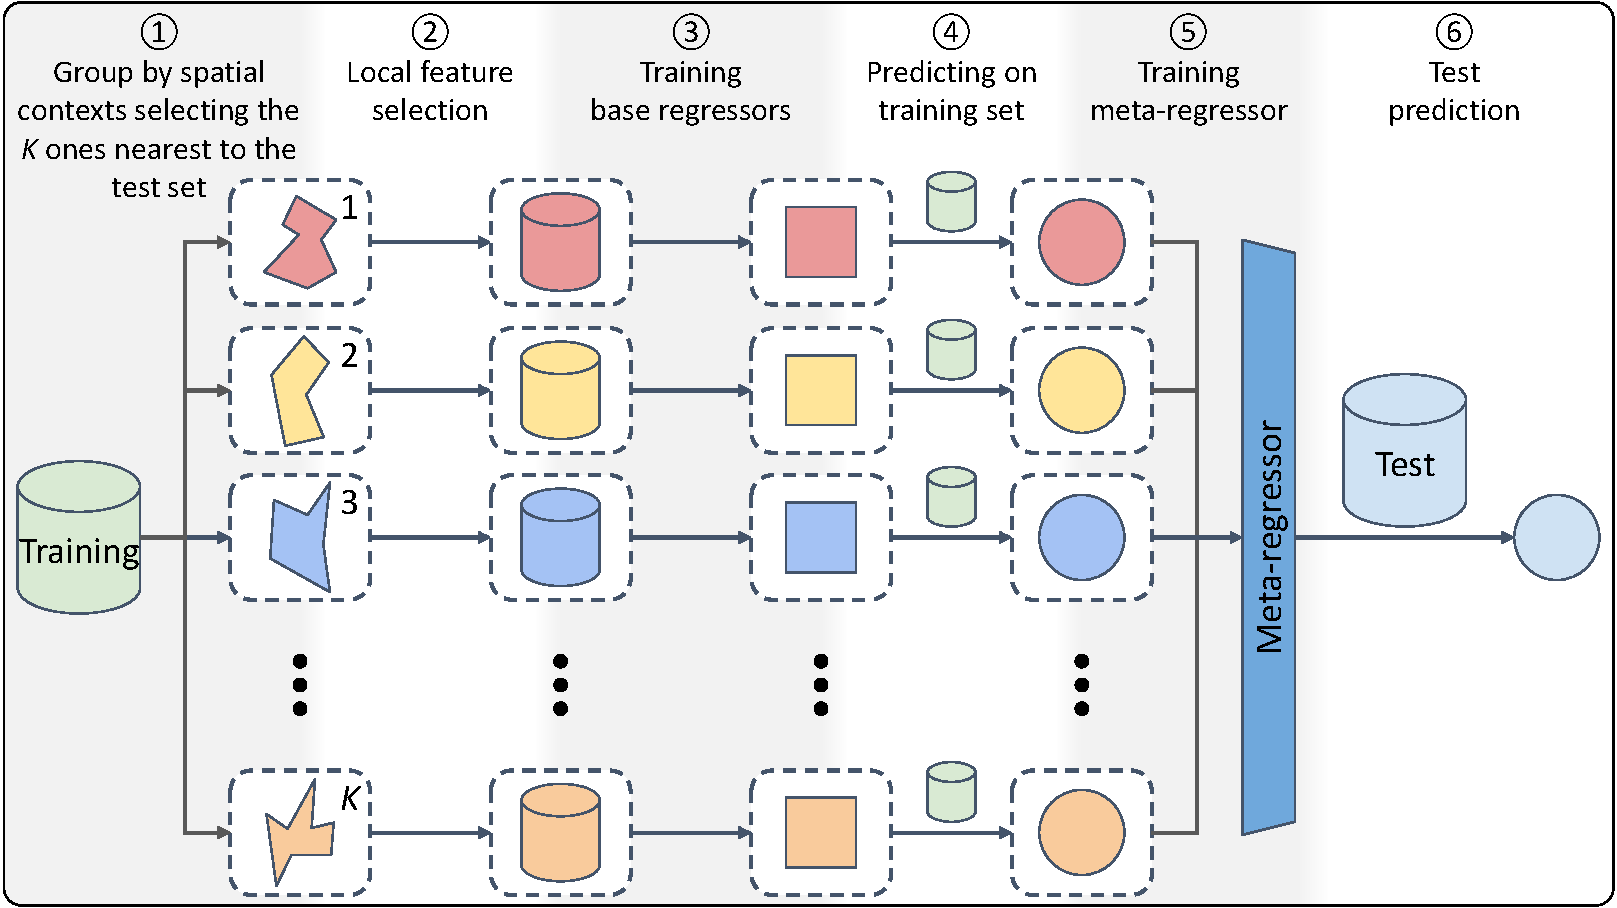
\includegraphics[width=0.94\linewidth]{approach.pdf}
    \caption{Proposed approach.}
    \label{fig:approach}
\end{figure}

Fig.~\ref{fig:approach} outlines the steps of our approach. In Step 1, we group the training data in agreement with a pre-defined set of spatial contexts and select the $K$ ones nearest to the test set, considering geographic proximity; the number of instances in each spatial context can vary. In Step 2, we run a feature selection method for each spatial context data, generating $K$ spatial context with different dimensions. In Step 3, we build an ensemble where each base regressor is fitted to a spatial context. In Step 4, we use the base regressors that make up the ensemble to predict the entire training set, creating an attribute-value table. In Step 5, we employ the data table to train a meta-regressor that will seek to ponder the local knowledge learned by the base regressors to maximize the generalization potential. Finally, in Step 6, the meta-regressor uses the predictions from the base regressors on the test set to provide final predictions.

As can be seen, our approach operates on two levels. The first level learns local patterns from geographically contextualized data samples, \textit{i.e.}, regions containing mutually exclusive instances described by an optimal feature subset. In a complementary way, the second level extracts global knowledge of the local patterns to predict a region of interest.


%%

\section{Case Study}
\label{sec:case_study}

In 2018, Brazilians went to the polls to vote for their president. The final result was 55.13\% for the Social Liberal Party (Jair Bolsonaro) and 44.87\% for the Worker's Party (Fernando Haddad). This election, however, was marked by a highly polarized environment and flooded by distrust in the voting system \cite{lucas2020}. Understanding outcomes in this context is essential to discuss the external factors influencing voting decisions and identify the geographic and socio-economic extensions of the processes that undermine democratic foundations.

%%

\subsection{Brazilian Election Data}
\label{subsec:data}

The dataset analyzed here expresses the second round of the 2018 Brazilian presidential election and portrays 5565 Brazilian municipalities. It has 3999 explanatory features that represents the 2010 census and one target feature, which is the vote share received by the winning party.

The census data was sourced from the Brazilian Institute of Geography and Statistics (\textit{IBGE}). The data is available to the public via anonymized aggregated features that describe population groups delimited by geospatial areas, \textit{e.g.} municipalities, which correspond to the aggregation level used in this study. To avoid erroneous results, we standardized all the features according to the city's population size or the number of domiciles.

We sourced the election data from the Superior Electoral Court (\textit{TSE}), which provides vote count results regarding each voting machine called ``\textit{boletim da urna}''. We aggregated the vote counts at a city level and calculated the vote shares as the percentual of valid votes for the winning party.

%%

\subsection{Machine Learning Approaches and Algorithms}
\label{subsec:approaches}

Standard econometric methods are not comparable with our approach. They often focus on regression analysis and employ data at higher aggregation to provide national-level predictions \cite{graefe2019accuracy}. The \textsc{Hierarchical GCNN} model \cite{li2019deep}, in turn, can be used as a representative of state-of-the-art applied machine learning research. We adopted this method parameterized according to the best results in \cite{li2019deep}, named variation 2. Furthermore, we considered city-level data as the prediction layer and state-level data to create the second aggregation layer. % However, our experimental setup differs from the one used to evaluate the \textsc{Hierarchical GCNN}, leading to a different performance. 

We also defined two baselines, \textsc{Global} and \textsc{Local Mean}, to be compared with our proposal, addressed from now on as \textsc{Local Meta}. \textsc{Global} is the conventional approach that selects features and fits models favoring global relationships. \textsc{Local Mean} is an ensemble of contextual models that employs the average as a fusion function to compose the final predictions. These baselines can help us understand in which situations \textsc{Local Meta} performs best and explain how the stacking strategy increases performance and improves generalization.

%\begin{itemize}
%    \item \textsc{Global:} is the conventional approach that selects the features and fits the models favoring global relationships. This baseline can inform us whether our approach based on local modeling improves performance compared to the traditional one.
%    \item \textsc{Local Mean:} is an ensemble of contextual models similar to ours. However, it uses the average as the voting system to generate the final prediction. This baseline can provide information on the advantage of using the stacking approach to improve performance and generalization.
%\end{itemize}

We investigated two configurations involving the number of spatial contexts~($K$) for \textsc{Local Mean} and \textsc{Local Meta}. The first uses all the contexts in the training set~($K=C$), while the second employs the seven closest contexts~($K=7$) to the prediction area. Note that $7$ is the mean of each context's neighbors. This configuration, in particular, aims to answer whether filtering contexts based on the prediction area proximity can enhance results.

Concerning the base regressors, we considered nine belonging to different machine learning paradigms. Table~\ref{tab:base_algorithms} lists these algorithms and their parameters. As the meta-regressor for \textsc{Local Meta}, we chose Ordinary Least Squares (OLS) since it is a simple and parameterless model. We adopted the Correlation-based Feature Selection (CFS) method to reduce the attribute space. CFS aims to find a minimal optimal subset of features that are highly correlated with the target and not very redundant with each other.

\begin{table}[!htbp]
	\centering
	\scriptsize
	\caption{Base regressors and their parameters. The acronyms not yet defined are: \textit{k}-Nearest Neighbors (\textit{k}NN), Least Absolute Shrinkage and Selection Operator (LASSO), Decision Tree (DT), Gradient Boosting DT (GBDT), Multiyear Perceptron (MLP), and Support Vector Regression (SVR).}
	\resizebox{\columnwidth}{!}{
	\begin{tabular}{lll}
	\hline
	Base regressor & Parameter & Value \\ \hline
	\textit{k}NN & Number of nearest neighbors ($k$) & $3$ \\
	OLS & --- & --- \\
	LASSO & Regularization strength ($\alpha$) & $1$ \\
	Ridge & Regularization strength ($\alpha$) & $1$ \\
	ElasticNet & Constant that multiplies the penalty terms ($\alpha$) & $1$ \\
	 & Mixing parameter ($l1\_ratio$) & $0.5$ \\
	DT & Split criterion & \textsc{Gini} \\
	GBDT & Number of boosted trees to fit ($n\_estimators$) & $100$ \\
	 & Learning rate ($\varepsilon$) & $0.1$ \\
	MLP & Hidden layers ($h$) & $1$ \\
	 & Hidden layer size ($n$) & $M/2$ \\
	 & Learning rate ($\varepsilon$) & $0.001$ \\
	SVR & Kernel & \textsc{RBF} \\
	 & Gaussian's width of the radial basis kernel function ($\sigma$) & $1/(M*X.var())$ \\
	 & Regularization parameter ($\mathbb{C}$) & 1 \\ \hline
	\end{tabular}}
	\label{tab:base_algorithms}
\end{table}

Finally, we defined the spatial contexts for the ensemble approaches as the 26 Brazilian states save the Federal District, which has only one city. This decision comprises the understanding that, at a higher level, stakeholders such as political scientists and journalists are more interested in analyzing the election results considering known spatial boundaries like states. %\cite{koeppen2021places}.

%%

\subsection{Evaluation Measures}
\label{subsec:measures}

We assessed the approaches described in Section~\ref{subsec:approaches} using four individual performance measures: Mean Squared Error~(MSE), Mean Error Standard Deviation~(MESD), SPearman correlation~(SP), and SPearman correlation Standard Deviation~(SPSD). MSE expresses the approaches' performance in predicting the correct vote-share scale, while MESD reflects their stability regarding MSE. MSE does not indicate whether the order of the achieved predictions matches those in the ground truth. That is, if city $A$ received more votes than city $B$, MSE does not tell us whether the approaches were able to capture this order. Thus, we employed SP to assess the order of the predictions yielded by the approaches. Finally, SPSD provides information on how SP is distributed over the folds.

We also applied a Multi-Criteria Performance Measure~(MCPM) \cite{Parmezan:2017} to combine the four metrics mentioned above and thus guide the choice of adequate approaches. MCPM reflects the sum of the total area of an irregular polygon whose vertices comprise individual performance indexes. In this work, lower total area values indicate better predictive performances. Unlike the MSE and Standard Deviation measures, in which resulting values must be minimized, SP~($\rho$) must be maximized. Hence, we applied the SP complement: $1 - \rho$.

To understand the predictive power of our proposal, we employed the SHapley Additive exPlanation (SHAP) Values technique to analyze the results in the best and worst fold scenarios \cite{lundberg2017unified}. SHAP Values is a unified measure of feature importance widely used to comprehend predictions made by models. We believe that examining it within the scope of our application is indispensable, as it can reveal biased models and avoid misinterpretations. Especially for our approach, SHAP Values can be employed in the meta and base regressors to explain the most important spatial contexts to predict a given fold and the most relevant features of that context.

%%

\subsection{Experimental Setup}
\label{subsec:experimental_setup}

Fig.~\ref{fig:experimental_setup} illustrates our experimental setup, which considers the space's role in evaluating models designed to predict election outcomes. As depicted in this figure, we used the dataset prepared in agreement with Section~\ref{subsec:data}~(Step 1) to assess the approaches parameterized according to Section~\ref{subsec:approaches}~(Step 2). We applied an SCV technique, which da Silva \textit{et al.} \cite{tiago2021graph} explicitly proposed for the application in question, to estimate the performance of the models~(Step 3). We reported these results via the evaluation metrics described in Section~\ref{subsec:measures}~(Step 4). This experimental protocol assesses the investigated approaches more rigorously, as it avoids overoptimistic results by reducing the spatial dependence between test and training sets. While our multi-criteria analysis compares these models taking into account two important characteristics -- the scale and the order of the vote shares --, our interpretability analysis is necessary to understand the patterns found and uncover biased models. %In summary, the evaluation process for a given fold starts by filtering the features using the CFS on the training set, which can be local or global, depending on the approach. Then the models are fitted based on the training set to predict the test, similar to the traditional Cross-Validation.
%\vspace{-.3cm}
\begin{figure}[!ht]
    \centering
    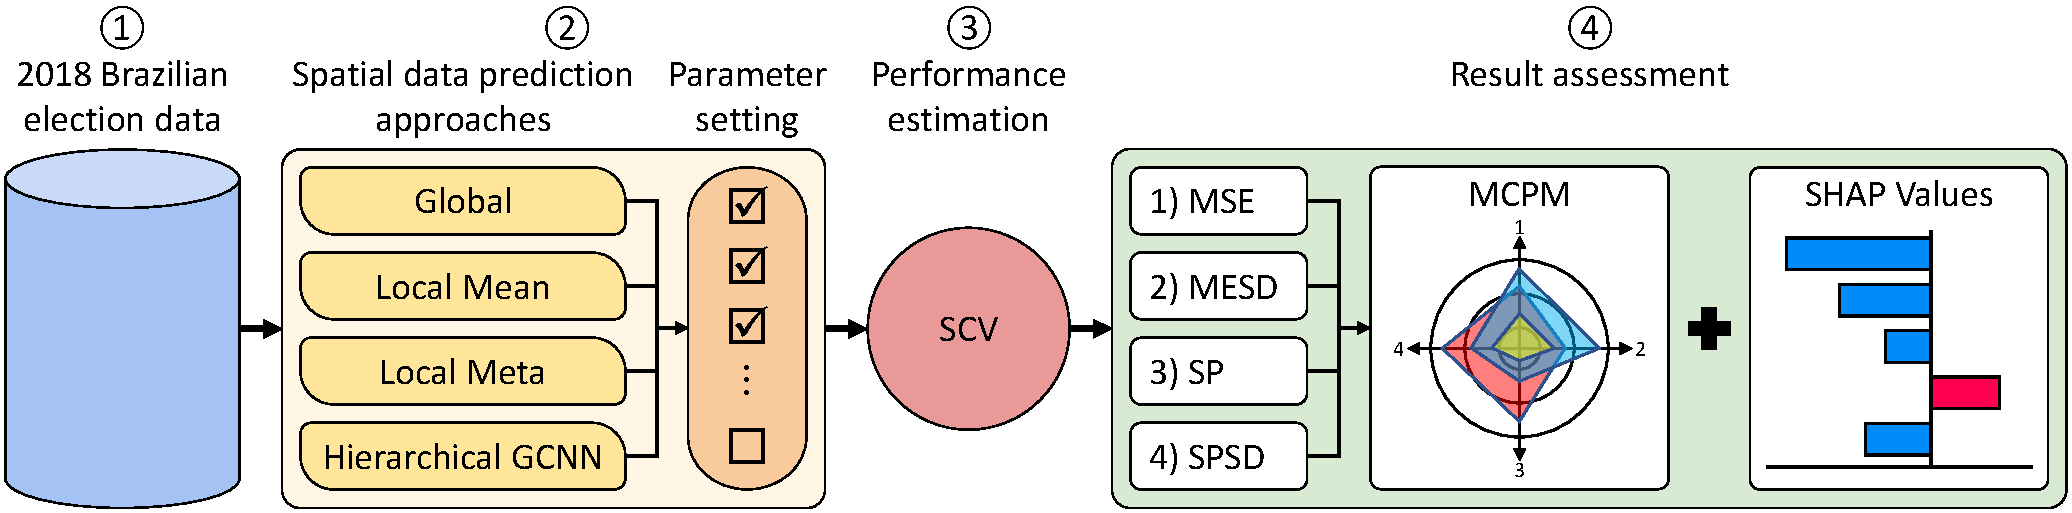
\includegraphics[width=0.98\linewidth]{experimental_setup.pdf}
    \caption{Experimental setup.}
    \label{fig:experimental_setup}
\end{figure}

The main difference between the SCV adopted in this work and the standard cross-validation lies in the fold definition so that in the former, the folds are determined based on preexisting geographic boundaries. Here, each spatial fold follows the geographic boundaries of the 26 Brazilian states, also employed as spatial contexts to build contextual base models in the ensemble approaches. Unlike the traditional cross-validation, in the SCV, the folds may have different distributions and sizes, creating a more challenging scenario for the approaches.

This study did not use folds 12 (Acre) and 13 (Rondonia) to calculate MSE and MSDE values because they present ambiguous distributions \cite{jiang2019spatial}; \textit{i.e.}, they describe a population with similar socio-economic characteristics to the northeastern but with vote shares similar to the southern states. This fact requires the approaches to learn the opposite of what they observed in the training set. Scenarios like these are challenging and exhibit incredibly high error rates, impacting empirical assessments, specifically the choice of the best regressor to compose \textsc{Global}. We decided to keep the analysis of SP and SPSD on such folds considering that the raised issue is linked to scale and not to order.

Finally, we implemented the experimental setup of Fig.~\ref{fig:experimental_setup} employing the Python programming language combined with the following libraries: Pandas, GeoPandas, SciPy, PySAL, and Scikit-learn. Our code and supplementary material are available on the GitHub platform\footnote{\url{https://github.com/tpinhoda/Spatial\_Context\_Stacking\_Approach}.}.


%%

\subsection{Results and Discussion}

As we can see from the averaged values of the individual performance metrics (Table~\ref{tab:overall_results}), \textsc{Local  Meta $K=7$} achieved the best MSE and MESD results, \textsc{Local Mean $K=C$} presented the highest SP values, and \textsc{Local Mean $K=7$} stood out in terms of SPSD. We obtained all these results using MLP as a base regressor. However, there was no consensus regarding the best model configuration -- approach and base regressor combination -- concerning all the metrics. To identify the most promising model, we evaluated the configurations under three perspectives: (i)~the MCPM to determine the best overall model; (ii)~the performance per fold to identify the best context-level configuration; (iii)~the model interpretability to understand the best configuration results.

\begin{table}[htbp]
	\centering
	\caption{Overall results of the approaches considering each base regressor and the following metrics: MSE, MESD, SP, and SPSD. Green cells symbolize the best results.}
	\resizebox{\columnwidth}{!}{
	\begin{tabular}{l|l!{\color{white}\vrule width 1pt}l!{\color{white}\vrule width 1pt}l!{\color{white}\vrule width 1pt}l|l!{\color{white}\vrule width 1pt}l!{\color{white}\vrule width 1pt}l!{\color{white}\vrule width 1pt}l|l!{\color{white}\vrule width 1pt}l!{\color{white}\vrule width 1pt}l!{\color{white}\vrule width 1pt}l|l!{\color{white}\vrule width 1pt}l!{\color{white}\vrule width 1pt}l!{\color{white}\vrule width 1pt}l|l!{\color{white}\vrule width 1pt}l!{\color{white}\vrule width 1pt}l!{\color{white}\vrule width 1pt}l}
	\hline
	 & \multicolumn{4}{c|}{\textsc{Global}} & \multicolumn{4}{c|}{\textsc{Local Mean K = All}} & \multicolumn{4}{c|}{\textsc{Local Mean K = 7}} & \multicolumn{ 4}{c|}{\textsc{Local Meta K = All}} & \multicolumn{4}{c}{\textsc{Local Mean K = 7}} \\
	 \multirow{-2}{*}{\parbox{1.5cm}{Base\\ regressors}} & \rotatebox[origin=l]{50}{MSE} & \rotatebox[origin=l]{50}{MESD} & \rotatebox[origin=l]{50}{SP} & \rotatebox[origin=l]{50}{SPSD} & \rotatebox[origin=l]{50}{MSE} & \rotatebox[origin=l]{50}{MESD} & \rotatebox[origin=l]{50}{SP} & \rotatebox[origin=l]{50}{SPSD} & \rotatebox[origin=l]{50}{MSE} & \rotatebox[origin=l]{50}{MESD} & \rotatebox[origin=l]{50}{SP} & \rotatebox[origin=l]{50}{SPSD} & \rotatebox[origin=l]{50}{MSE} & \rotatebox[origin=l]{50}{MESD} & \rotatebox[origin=l]{50}{SP} & \rotatebox[origin=l]{50}{SPSD} & \rotatebox[origin=l]{50}{MSE} & \rotatebox[origin=l]{50}{MESD} & \rotatebox[origin=l]{50}{SP} & \rotatebox[origin=l]{50}{SPSD} \\ \hline
	\textit{k}NN & 239.68 & 267.93 & 0.46 & 0.16 & 272.04 & 187.92 & 0.58 & 0.15 & 303.78 & 216.51 & 0.50 & 0.17 & 179.50 & 157.93 & 0.56 & 0.17 & 173.60 & 162.65 & 0.51 & 0.17 \\
	OLS & 121.81 & 134.17 & 0.59 & 0.15 & 271.08 & 197.79 & 0.60 & 0.19 & 219.96 & 170.12 & 0.59 & 0.13 & 224.67 & 195.01 & 0.55 & 0.20 & 125.81 & 141.26 & 0.57 & 0.13 \\
	LASSO & 965.26 & 465.45 & 0.02 & 0.50 & 949.42 & 457.43 & 0.38 & 0.24 & 949.24 & 456.68 & 0.26 & 0.24 & 876.07 & 405.93 & 0.35 & 0.25 & 837.60 & 427.85 & 0.27 & 0.25 \\
	Ridge & 304.48 & 194.94 & 0.58 & 0.16 & 355.77 & 214.79 & \cellcolor[HTML]{6aa84f}\textcolor{white}{0.64} & 0.12 & 428.35 & 247.88 & 0.62 & 0.13 & 124.69 & 129.78 & 0.57 & 0.16 & 132.77 & 128.39 & 0.61 & 0.14 \\
	ElasticNet & 964.61 & 465.43 & 0.23 & 0.29 & 961.42 & 463.94 & 0.48 & 0.27 & 961.99 & 464.01 & 0.36 & 0.35 & 299.24 & 216.62 & 0.50 & 0.21 & 528.13 & 317.23 & 0.43 & 0.34 \\
	DT & 269.36 & 355.57 & 0.32 & 0.22 & 223.96 & 178.53 & 0.52 & 0.17 & 287.03 & 232.21 & 0.41 & 0.19 & 213.99 & 189.83 & 0.48 & 0.19 & 230.87 & 201.68 & 0.43 & 0.19 \\
	GBDT & 171.56 & 159.91 & 0.51 & 0.17 & 196.32 & 153.97 & 0.61 & 0.16 & 249.46 & 186.00 & 0.56 & 0.17 & 159.09 & 149.73 & 0.54 & 0.18 & 142.39 & 140.13 & 0.56 & 0.18 \\
	MLP & 133.87 & 138.18 & 0.61 & 0.14 & 240.22 & 170.30 & \cellcolor[HTML]{6aa84f}\textcolor{white}{0.64} & 0.13 & 311.43 & 207.35 & 0.62 & \cellcolor[HTML]{6aa84f}\textcolor{white}{0.12} & 127.01 & 132.60 & 0.57 & 0.17 & \cellcolor[HTML]{6aa84f}\textcolor{white}{111.22} & \cellcolor[HTML]{6aa84f}\textcolor{white}{127.19} & 0.59 & 0.14 \\
	SVR & 243.97 & 206.58 & 0.55 & 0.18 & 398.58 & 238.68 & 0.62 & 0.14 & 447.63 & 261.98 & 0.59 & 0.15 & 168.97 & 149.09 & 0.52 & 0.23 & 164.13 & 146.32 & 0.55 & 0.18 \\ \hline
	\end{tabular}
	\label{tab:overall_results}}
\end{table}

%%

\subsubsection{Multi-Criteria Performance} 
\label{subsec:mcpm}

Fig.~\ref{fig:mcpm} shows, for each approach configuration, the MCPM values ranked in descending order of importance. \textsc{Local Meta $K=7$} presented a more consistent behavior occupying the first and second positions for most configurations, with its lowest position being the third employing DT. On the other hand, the \textsc{Global} and \textsc{Local Meta $K=C$} approaches exhibited high variance across the multi-criteria ranks, indicating a sensibility to the choice of the base regressor. Furthermore, the ensemble approaches that adopted the average-based voting strategy (\textsc{Local Mean $K=C$}  and \textsc{Local Mean $K=7$}) yielded the poorest MCPM values, occupying the fourth and fifth positions for most configurations.
%\vspace{-.3cm}
\begin{figure}[!ht]
    \centering
    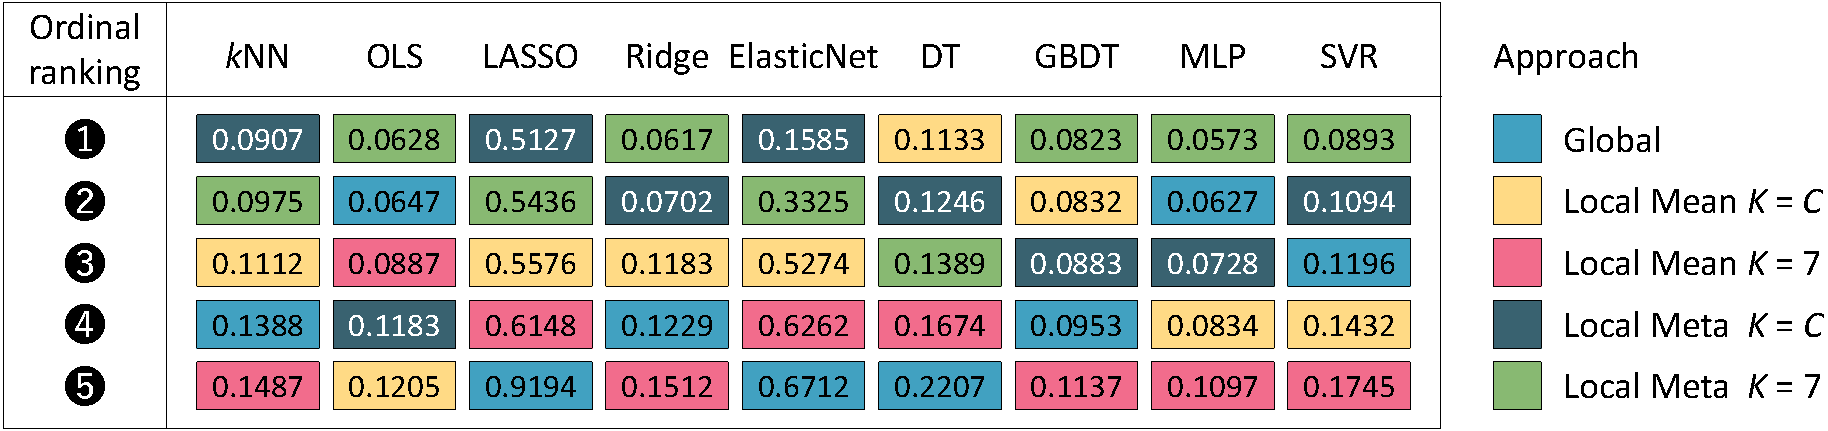
\includegraphics[width=0.98\linewidth]{mcpm.pdf}
    \caption{MCPM values ranked in descending order of importance for each approach regarding different base regressors.}
    \label{fig:mcpm}
\end{figure}

To compare our proposal and the baseline approaches with the state-of-the-art model, we selected their best configurations in terms of base regressors and arranged their results in Table~\ref{tab:best_approaches_configurations}. \textsc{Local Meta $K=7$} achieved the best performances in four out of five metrics, including MCPM, and presented the second-best SP result. \textsc{Hierarchical GCNN}, in turn, presented the worst performance across all the metrics. We must emphasize that the method had parameter values following the best results reported in \cite{li2019deep}, which considered the 2019 Australian election and the traditional cross-validation. Therefore, the present work did not apply a fine-tuning step for \textsc{Hierarchical GCNN} since it is not a step performed in our experimental protocol.

%\textsc{Hierarchical GCNN}, in turn, presented the worst performance across all the metrics. We must emphasize that our experimental setup differs from the one where the approach was originally proposed \cite{li2019deep}. We consider the 2018 Brazilian Presidential Election and the SCV as the validation technique. Thus, it is not a fair comparison since they found their best parameters in a different scenario. Therefore, the approach requires a fine-tuning step to achieve better results, which is not a step performed in this work since we did not apply fine-tuning to any of the base regressors used in this paper.

%\textsc{Hierarchical GCNN}, in turn, presented the worst performance across all the metrics. We must emphasize that the experimental setup used to evaluate this approach in its proposing paper differs from ours.We used a dataset from another election and a different validation technique. Thus, it is not a fair comparison since they found their best parameters in a different scenario. Therefore, the approach requires a fine-tuning step to achieve better results, which is not a step performed in this work since we did not apply fine-tuning to any of the base regressors used in this paper.

\definecolor{my_green}{HTML}{6aa84f}
\begin{table}[htbp]
	\centering
	\scriptsize
	\caption{Most promising approaches based on overall configuration performances. Green cells denote the best results.}
	\resizebox{\columnwidth}{!}{
	\begin{tabular}{l!{\color{white}\vrule width 1pt}l!{\color{white}\vrule width 1pt}l!{\color{white}\vrule width 1pt}l!{\color{white}\vrule width 1pt}l!{\color{white}\vrule width 1pt}l!{\color{white}\vrule width 1pt}l}
	\hline
	Approach & Base regressor & MSE & MESD & SP & SPSD & MCPM \\ \hline
	\textsc{Global} & MLP & 133.87114 & 138.17511 & 0.5907 & 0.1531 & 0.0681 \\
	\textsc{Local Mean $K=C$} & GBDT & 196.31742 & 153.97060 & \cellcolor[HTML]{6aa84f}\textcolor{white}{0.6090} & 0.1560 & 0.0832 \\
	\textsc{Local Mean $K=7$} & OLS & 219.95581 & 170.12371 & 0.5850 & 0.1298 & 0.0887 \\
	\textsc{Local Meta $K=C$} & Ridge & 124.69428 & 129.78054 & 0.5701 & 0.1646 & 0.0702 \\
	\textsc{Local Meta $K=7$} & MLP & \cellcolor[HTML]{6aa84f}\textcolor{white}{111.22174} & \cellcolor[HTML]{6aa84f}\textcolor{white}{127.19046} & 0.5911 & \cellcolor[HTML]{6aa84f}\textcolor{white}{0.1355} & \cellcolor[HTML]{6aa84f}\textcolor{white}{0.0573} \\
	\textsc{Hierarchical GCNN} & GCNN & 229.11080 & 209.11220 & 0.4917 & 0.1822 & 0.1279 \\ \hline
	\end{tabular}}
	\label{tab:best_approaches_configurations}
\end{table}

In summary, our approach proved to be more stable against base regressors from different paradigms than the baselines. Additionally, \textsc{Local Meta $K=7$} configured with MLP culminated in the best overall results compared to the best configurations of the other approaches. 

%%

\subsubsection{Performance per Fold}

Fig.~\ref{fig:statistics_per_fold} displays the fold-level results of the best-instantiated approaches indicated in Table~\ref{tab:best_approaches_configurations}. The performances are reported according to MSE, MESD, and SP. We disregard the SPSD metric here since we cannot produce its values per fold.

\begin{figure}[!ht]
    \centering
    \subfigure[MSE per fold]{
        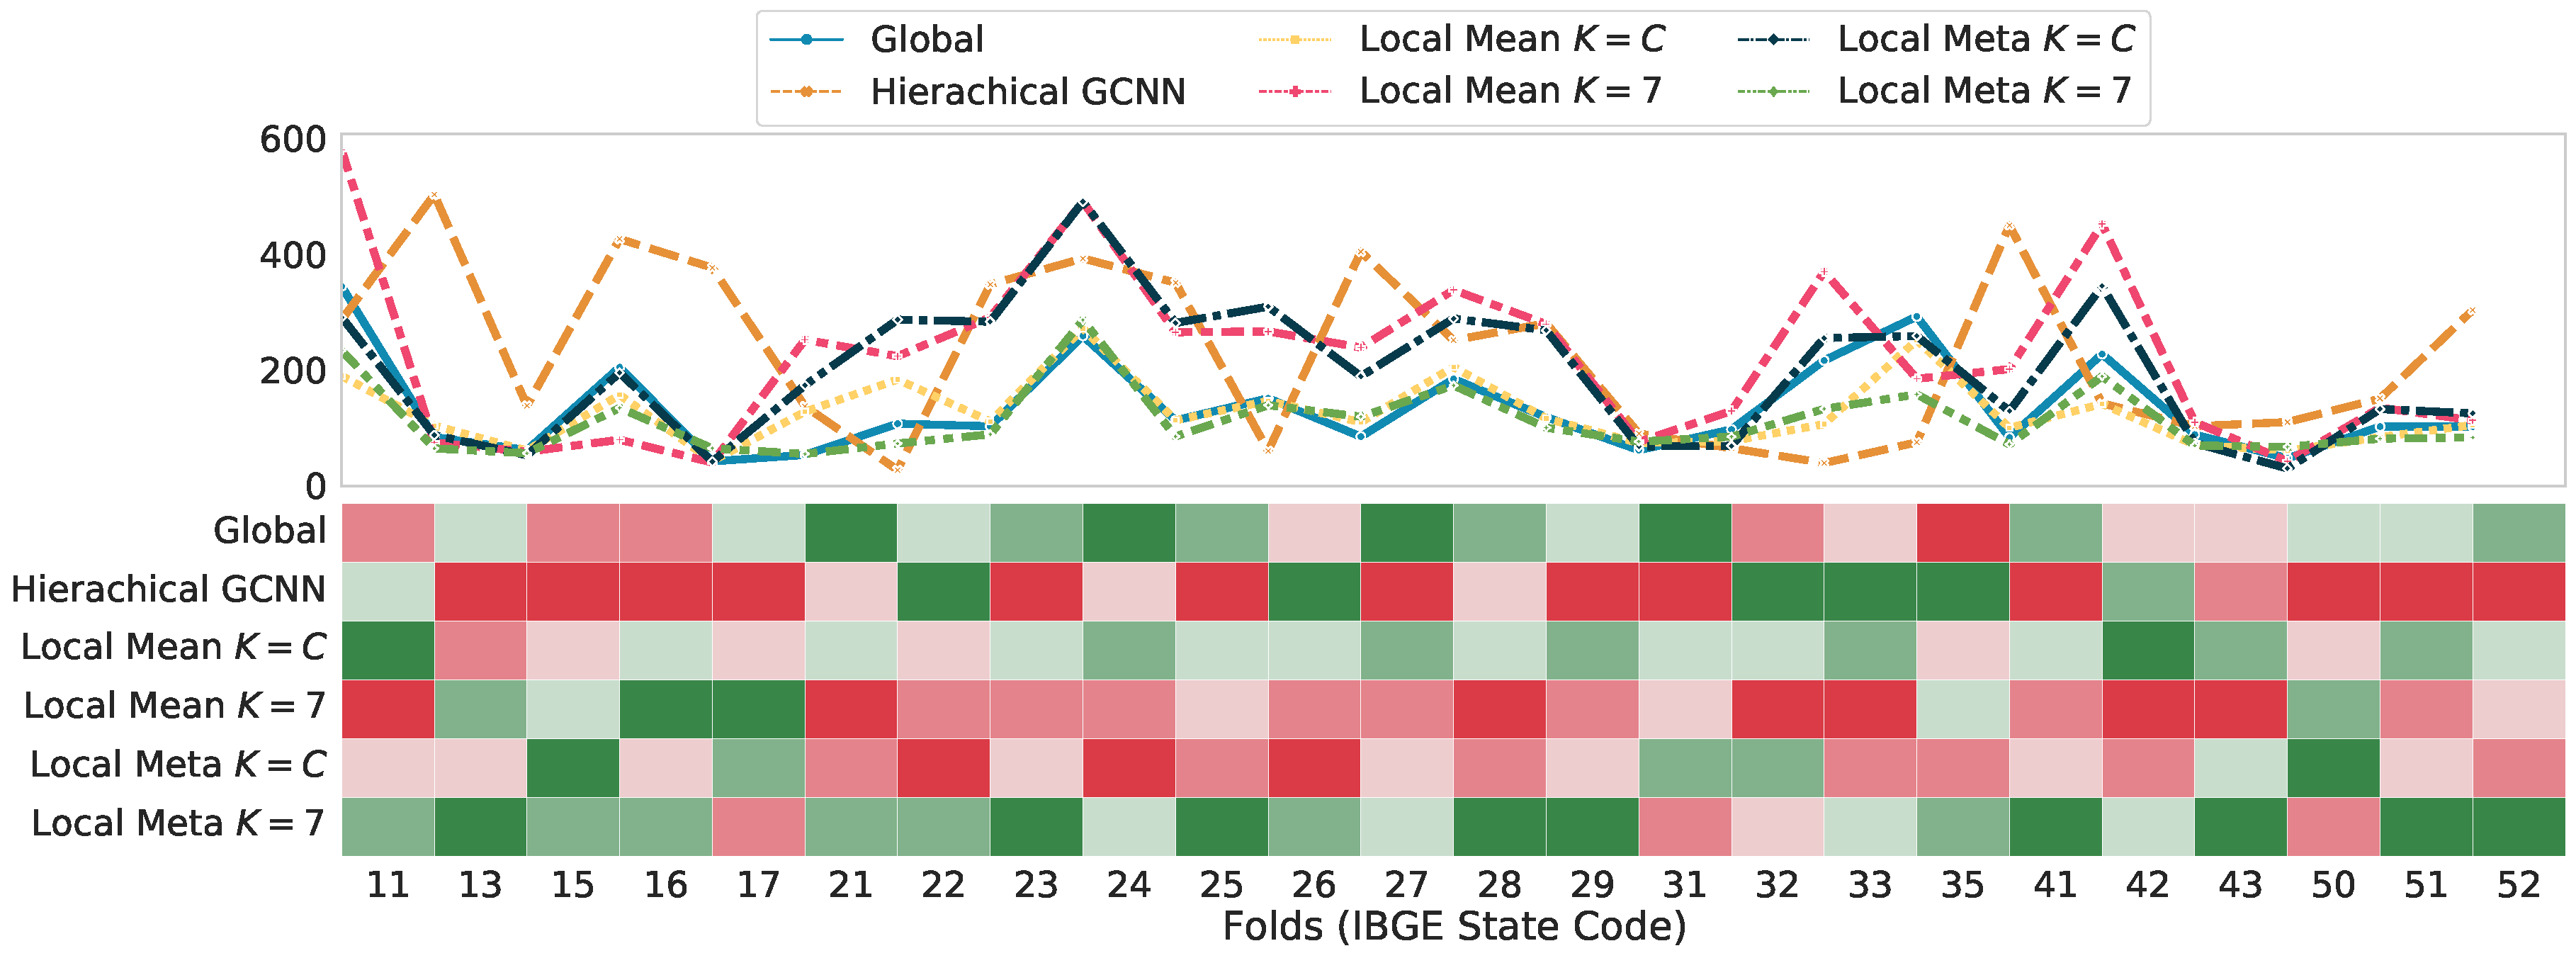
\includegraphics[page=1,width=0.96\linewidth]{metrics.pdf}
        \label{subfig:mse}
    }
    \qquad
    \subfigure[MESD per fold]{
        \includegraphics[page=2,width=0.96\linewidth]{metrics.pdf}
        \label{subfig:mesd}
    }
    \qquad
    \subfigure[SP per fold]{
        \includegraphics[page=3,width=0.96\linewidth]{metrics.pdf}
        \label{subfig:sp}
    }
    \caption{Metrics per fold coming from the approaches whose configurations were considered the best by MCPM.}
    \label{fig:statistics_per_fold}
\end{figure}

Concerning MSE (Fig.~\ref{subfig:mse}) and MESD (Fig.~\ref{subfig:mesd}), \textsc{Local Meta $K=7$} behaved stably over the folds, followed by \textsc{Global}. \textsc{Local Meta $K=7$} also achieved the best results on most folds, performing exceptionally well in the northeastern states (samples 21 to 29), where it exhibited the best or second best MSE and MESD. Folds 17, 31 and 50, for which \textsc{Local Meta $K=7$} was ranked lower regarding MSE, demonstrated close values. Thus, there was no discrepant difference between the investigated approaches. We observed the same in folds 16, 17, and 30 concerning MESD.

%Concerning the MSE metric, Fig.~\ref{subfig:mse} presents two high peaks corresponding to folds 12 (Acre) and 13 (Rondonia). These folds present unseen uncorrelated distributions, that is, there is no similar distribution in the training set. In other words, they present a population with similar socio-economic characteristics to the northeastern and northern states but with vote shares similar to the southern states. These circumstances pose a challenging scenario for all approaches since it requires the models to learn the opposite of what they observed in the training set. On the other hand, regarding the remaining folds, the two variations of our approach presented a closer behavior when compared to the \textit{Global} approach with slightly lower values of MSE in the northern (folds 21-29) and southern (folds 31-35) states. 

In terms of SP (Fig.~\ref{subfig:sp}), the \textsc{Global} approach obtained better results than the two variations of our proposal in most folds. However, it was closely followed by \textsc{Local Meta $K=7$}, specifically in the northeastern states (samples 21 to 29). This fact is reinforced by both approaches' relatively close average performances (\textsc{Global}: $0.61$; \textsc{Local Meta $K=7$}: $0.59$).

%Finally, the average rank per fold (Figure \ref{fig:rank}) indicates that the \textit{Local Meta $K=7$} achieved the lowest MSE in 12 out of 26 folds, followed by the \textit{Global} and \textit{Local Meta $K=All$} that presented the lowest MSE in 4 folds, while the \textit{Local Mean} approaches reached first place in 3 folds each. Thus, despite the \textit{Local Meta $K=7$} having presented a higher average MSE  when compared to \textit{Local Meta $K=All$}, it produced better results in almost half of the folds.

As we can see, the per-fold analysis of the three individual performance measures corroborates the one guided by MCPM, indicating that the two variations of our approach perform better than the other baseline models. Our proposal exhibited better MSE and MESD results than the other approaches. However, despite presenting lower SP values when compared with \textsc{Global}, the two variations of our proposal showed close results in most folds and performed better in some folds from the Southeast and Northeast.

%%

\subsubsection{Model Interpretability}

%In this section, we aim to understand the predictions assigned by the best configurations for the two variations of our approach (\textit{Local Meta $K=All (Ridge)$} and \textit{Local Meta $K=7$ (MLP)}). We use the SHAP values to identify if there is a bias in the approaches that could cause misinterpretation and to comprehend the features' importance in the predictions.

%The first analysis regards the meta-regressor and seeks to understand how the meta-model assigned importance to the spatial context when predicting the folds. In Fig.~\ref{fig:count_most_importante_context} we showed the number of times each spatial context was chosen as the most important during the SCV evaluation process. The \textit{Local Meta $K=All (Ridge)$} chose the spatial context 35 (São Paulo) as the most important context for 15 out of 26 folds and the spatial context 25 (Ceará) as the most important for 8 folds. This result shows a biased behavior, where the approach uses only two spatial contexts as the most important to predict the other 24 folds. On the other side, the \textit{Local Meta $K=All (Ridge)$} presented a more distributed set of most important contexts that covers all the regions of Brazil. Such characteristic makes the approach more realistic, having more potential to explain the regional aspects of each fold.

%\begin{figure}[!ht]
%    \centering
%    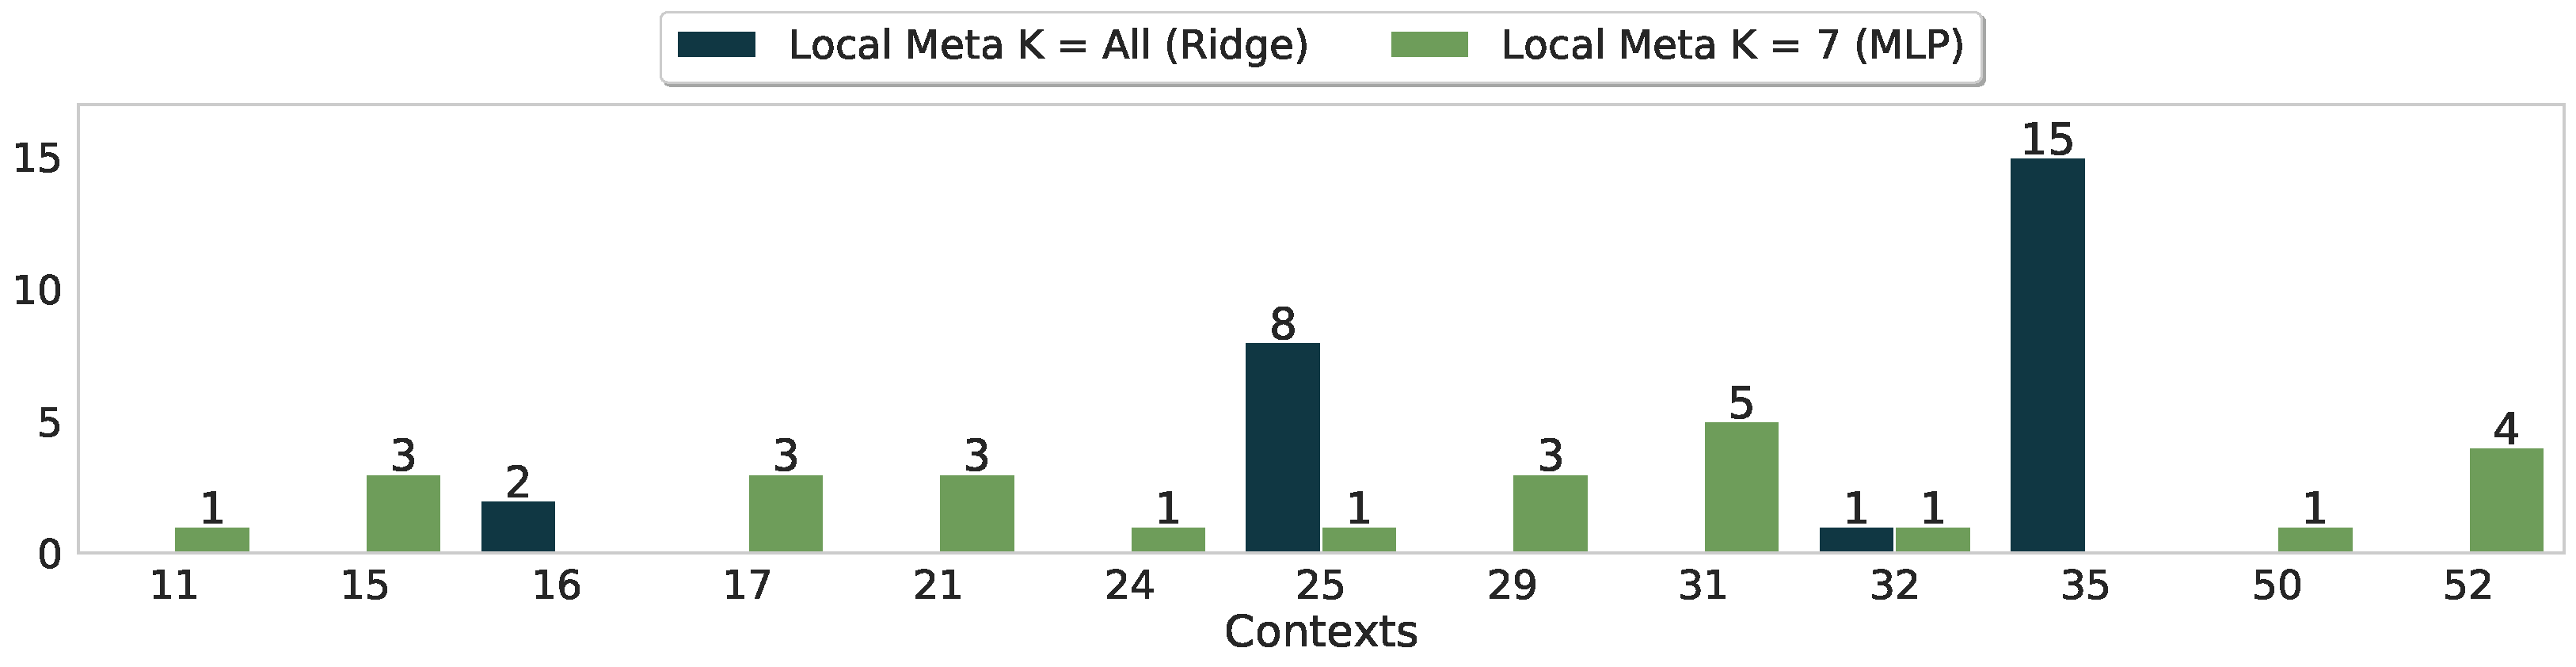
\includegraphics[page=1, width=\linewidth]{shap_values.pdf}
%    \caption{The number of times each context was chosen as the most important according to the meta-regressor SHAP Values. Spatial contexts not presented in the plot had zero counts.}
%    \label{fig:count_most_importante_context}
%\end{figure}

Aiming to understand the predictions assigned by the best approach configuration (\textsc{Local Meta $K=7$} with MLP), we considered the SHAP Values technique to produce an in-depth interpretability analysis. We sought to understand the most important context and the most important relevant features from this context in the best (sample 23 or Maranhão) and worst (sample 16 or Amapá) folds regarding MSE. Figs.~\ref{fig:shap_values_best_case} and \ref{fig:shap_values_worst_case} comprise four plots. The first is the actual vote share distribution, while the second is the predicted distribution. The third concerns the feature importance given by the meta-regressor for each spatial context when predicting the fold. The fourth and last plot presents the top-five most relevant features according to the base regressor fitted to the most important context. Besides, Tables~\ref{tab:best_case_top_five_feaures_description} and \ref{tab:worst_case_top_five_feaures_description} list the top-five most important features of Figs.~\ref{fig:shap_values_best_case} and \ref{fig:shap_values_worst_case}, respectively.

\begin{figure}[!ht]
    \centering
    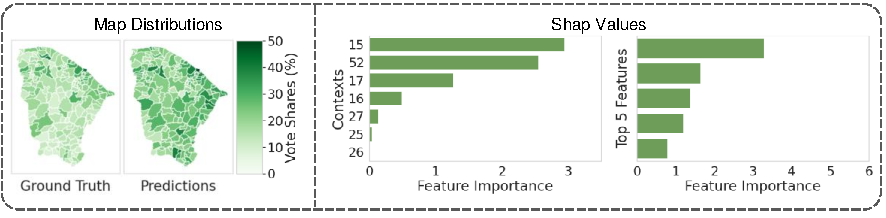
\includegraphics[page=1, width=\linewidth]{shap_values_lv.pdf}
    \caption{Vote share distribution and SHAP Values for the best-case scenario (fold 23) in terms of \textsc{Local Meta $K=7$} with MLP. The plots cover, from left to right, the following information: (a.1) actual vote share distribution, (a.2) predicted vote share distribution, (b.1) feature importance given by the meta-regressor for each spatial context, and (b.2) top-five most relevant features according to the base regressor fitted to the most important context (sample 15). The feature names are presented in the same order as in Table~\ref{tab:best_case_top_five_feaures_description}.}
    \label{fig:shap_values_best_case}
\end{figure}
Concerning the best-case scenario (Fig.~\ref{fig:shap_values_best_case}), our approach predicted vote shares slightly above the actual values, observed by the number of dark regions in the prediction map in relation to the ground-truth map. The meta-regressor chose the geographic context 15 (Amazonas) as the most important, and the most relevant feature from context 15 was \texttt{PessoaRenda V045}. The selection of Amazonas as the most important context to predict the vote shares in Maranhão is coherent since both states present similar vote shares and related socio-economic characteristics. We should note that the first and third most relevant features from context 15 describe the women with income per capita less than half of the minimum wage (Table~\ref{tab:best_case_top_five_feaures_description}). This result is in line with research that points to the relationship between low-income women and lower votes for the winning party in the 2018 Brazilian presidential election \cite{layton2021demographic,pinheiro2020hope}. The remaining characteristics still need to be carefully analyzed to verify if they are proxies for other known related features such as poverty (\texttt{Domicilio02 V057} and \texttt{Domicilio02 V052}) or a local relationship (\texttt{Entorno05 V977}).

\begin{table}[htbp]
	\centering
	\scriptsize
	\caption{Top-five features from the most important context in the best-case scenario~(fold 23).}
	\resizebox{\columnwidth}{!}{
	\begin{tabular}{l|p{10cm}}
	\hline
	Feature &  Description \\ \hline
	\texttt{PessoaRenda V045} &  Women over ten years with a nominal monthly income of up to half minimum wage \\
	\texttt{Domicilio02 V057} &  Men living in permanent private households with water supply from a well or spring on the property \\
	\texttt{ResplRenda V055} &  Total nominal monthly income of responsible women with a nominal monthly income of up to 1/2 minimum wage \\
	\texttt{Domicilio02 V052} &  Men residing in rented permanent private homes \\
	\texttt{Entorno05 V977} &  Asian residents in permanent private homes with street lighting \\ \hline
	\end{tabular}}
	\label{tab:best_case_top_five_feaures_description}
\end{table}

In the worst-case scenario (Fig.~\ref{fig:shap_values_worst_case}), our approach predicted much higher vote shares than the ground truth, especially in the northern region. The meta-regressor chose context 24 (Rio Grande do Norte) as the most important, and the most relevant feature from context 24 was \texttt{Entorno04 V490} followed close by \texttt{Domicilio02 V040}. The selection of Rio Grande do Norte as the most important context to predict the vote shares in Amapá was not a good decision, given the high error rates. Its features were insufficient to provide a good performance and cannot deliver insights into Amapá's voting results. We can see from Table~\ref{tab:worst_case_top_five_feaures_description} that most of the top-five relevant features describe particularities related to rural regions of context 24. These proprieties may not be observed in fold 16 or present a different relationship with the target, causing the approach performance to deteriorate. %However, further analysis should be conducted to provide more information regarding these results.

\begin{figure}[!ht]
    \centering
    \includegraphics[page=2, width=\linewidth]{shap_values_lv.pdf}
    \caption{Vote share distribution and SHAP Values for the worst-case scenario (fold 16) in terms of \textsc{Local Meta $K=7$} with MLP. The plots cover, from left to right, the following information: (a.1) actual vote share distribution, (a.2) predicted vote share distribution, (b.1) feature importance given by the meta-regressor for each spatial context, and (b.2) top-five most relevant features according to the base regressor fitted to the most important context (sample 24). The feature names are presented in the same order as in Table~\ref{tab:worst_case_top_five_feaures_description}.}
    \label{fig:shap_values_worst_case}
\end{figure}

Despite the challenge in modeling local relationships from socio-economic and election data, the in-depth assessment of SHAP Values indicated that our proposal is intelligible and, at best, predictions are based on coherent features that can aid in understanding electoral outcomes.

\begin{table}[htbp]
	\centering
	\scriptsize
	\caption{Top-five features from the most important context in the worst-case scenario~(fold 16).}
	\resizebox{\columnwidth}{!}{
	\begin{tabular}{l|p{10cm}}
	\hline
	Feature &  Description \\ \hline
	\texttt{Entorno03 V490} &  Number of residents in private households without permanent public lighting with a well or spring on the property \\
	\texttt{Domicilio02 V040} &  Residents in permanent private households with electricity from other sources \\
	\texttt{Domicilio01 V026} &  Permanent private homes with two bathrooms for the exclusive use of residents \\
	\texttt{Domicilio01 V162} &  Permanent private dwellings, such as village houses or condominiums, without a bathroom for the exclusive use of residents \\
	\texttt{Entorno04 V730} &  Residents without nominal monthly household income per capita in permanent private households without sidewalks \\ \hline
	\end{tabular}}
	\label{tab:worst_case_top_five_feaures_description}
\end{table}

\section{Conclusion}
\label{sec:conclusion}

This work proposed a geographic context-based stacking learning approach to predict election outcomes using socio-economic features. Our model is built in levels and dynamically selects contexts according to a data sample we want to predict. This modeling allows the generation of more realistic descriptive models whose relationships enable a more accurate understanding of voting behavior. We also introduced a spatial cross-validation-driven experimental setup to fairly assess and compare geographically contextualized approaches. Despite the challenging nature of the problem, by considering the second round of the 2018 Brazilian presidential election, our proposal experimentally showed promising results, including intelligible and coherent predictions in the best-case scenario and stable performance over the remaining folds compared with the reference models.

However, there is still room for further improvement. Our approach does not deal with ambiguous distributions, an aspect that often appears in modeling voting behavior. Furthermore, this paper was restricted to analyzing a single dataset, and studies with other election databases may be beneficial. Sophisticated machine learning methods such as Graph Neural Networks should also be better evaluated as they have shown satisfactory results for spatial data.


% ---- Bibliography ----
%
% BibTeX users should specify bibliography style 'splncs04'.
% References will then be sorted and formatted in the correct style.
%
\bibliographystyle{splncs04}
\bibliography{bibliography}
%

\end{document}
